\documentclass[tikz,border=8pt]{standalone}
\usepackage{tikz}
\usepackage{tkz-euclide}
\usepackage{amsmath, amssymb}

\usetikzlibrary{angles, quotes}

\begin{document}

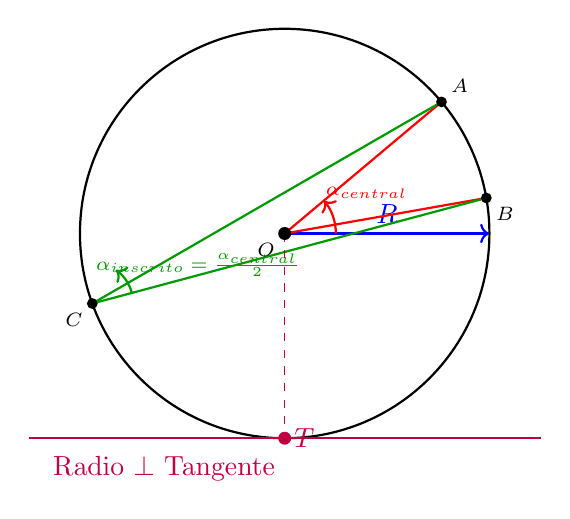
\begin{tikzpicture}[scale=1.3]

  % ---- Circunferencia ----
  \coordinate (O) at (0,0);
  \draw[thick] (O) circle (2);

  % ---- Radio ----
  \draw[blue, thick, ->] (O) -- (0:2) node[midway, above] {$R$};

  % ---- Ángulo central (en O) ----
  \coordinate (A) at (40:2);
  \coordinate (B) at (10:2);
  \draw[red, thick] (O) -- (A);
  \draw[red, thick] (O) -- (B);
  \draw[->, red, thick] (0.5,0) arc (0:40:0.5);
  \node[red] at (0.8,0.4) {\scriptsize $\alpha_{central}$};

  % ---- Ángulo inscrito (en C sobre la circunferencia) ----
  \coordinate (C) at (200:2);
  \draw[green!60!black, thick] (C) -- (A);
  \draw[green!60!black, thick] (C) -- (B);
  \draw[->, green!60!black, thick] (C) ++(15:0.4) arc (15:55:0.4);
  \node[green!60!black] at ($(C)!0.55!(0,0)$) {\scriptsize $\alpha_{inscrito}=\frac{\alpha_{central}}{2}$};

  % ---- Recta tangente en T ----
  \coordinate (T) at (270:2);
  \draw[purple, thick] (2.5,-2) -- (-2.5,-2);
  \draw[purple, dashed] (O) -- (T);
  \node[purple, right] at (T) {$T$};
  \node[purple, left] at (0,-2.3) {Radio $\perp$ Tangente};

  % ---- Puntos etiquetados ----
  \fill (O) circle (1.8pt) node[below left] {\scriptsize $O$};
  \fill (A) circle (1.5pt) node[above right] {\scriptsize $A$};
  \fill (B) circle (1.5pt) node[below right] {\scriptsize $B$};
  \fill (C) circle (1.5pt) node[below left] {\scriptsize $C$};
  \fill[purple] (T) circle (1.8pt);

\end{tikzpicture}

\end{document}
